
\section{Finanzplanung}
Hier erläutern wir die Hauptkostenarten sowie Einnahmequellen und entsprechende Annahmen, mit deren Hilfe wir zu einer realistischen Einschätzung der Cashflows der ersten zwei Jahre gelangen.
\subsection{Umsatz}
Als Umsatz werden für die Schätzung lediglich die Einnahmen aus den Abbonnements betrachtet. Zusätzlich sollten an dieser Stelle auch Werbeeinnahmen addiert werden, die wir jedoch mangels genauer Prognosen weglassen. Es handelt sich hier also um eine konservative Schätzung.\\
Neben den kalkulierten Preisen für private Accounts (1\euro basic, 3\euro extended) und Firmenkunden (150\euro basic, 450\euro extended) nehmen wir außerdem je Kundengruppe einen Split von 30-70 für den Kauf der extended- bzw. der basic-Version an. Der Marktanteil wird konservativ mit 1\% angesetzt, was einer realistischen Schätzung für ein Spezial-Start-Up in den ersten 24 Monaten entspricht.
\subsection{Hauptkostenarten}
Im ersten Monat fallen Lizenzkosten in Höhe von 35.000\euro an. Dazu kommen relativ geringfügige Fixkosten der GmbH-Anmeldung. In den darauf folgenden 4 Monaten spielen die Kosten des externen Development-Dienstleisters eine wichtige Rolle. \\
Den bei weitem größten laufenden Posten bilden die Personalkosten, gefolgt von den variablen Kosten der IT-Infrastruktur bei Amazon Web Services. 

\subsection{Szenario-Analyse}
Ausgehend von dem Normalfall werden das beste und schlechteste Szenario simuliert, indem die Umsatzerlöse variiert werden. Die Kosten nehmen wir dabei jeweils als konstant an.\\
Für jedes Szenario ist die Lage des Break-Even Punktes von Interesse:
\\
\\
\begin{table}[h!]
  \centering
    \begin{footnotesize}
  \begin{tabular}{|l|l|l|l|}\hline
  \textbf{ } &  \textbf{Umsatz (relativ)} &  \textbf{Break-Even} \\ \hline
 \textbf{best case} & 150\% & 12. Monat \\ \hline
\textbf{neutral case} & 100\% & 18. Monat \\ \hline
 \textbf{worst case} & 50\% & 25. Monat \\ \hline
  \end{tabular} 
    \end{footnotesize}
  \caption{Break-Evene in Szenarien mit unterschiedlicher Umsatzentwicklung}
  \label{tab:break-even}
\end{table} 

\begin{figure}[h!]
\centering
\includegraphics[width=0.9\textwidth]{financials}
\caption{Finanzplan im neutralen Fall}
\label{fig:financials1}
\end{figure}

\subsection{Detaillierte Finanzplanung}



\begin{figure}[h!]
\centering
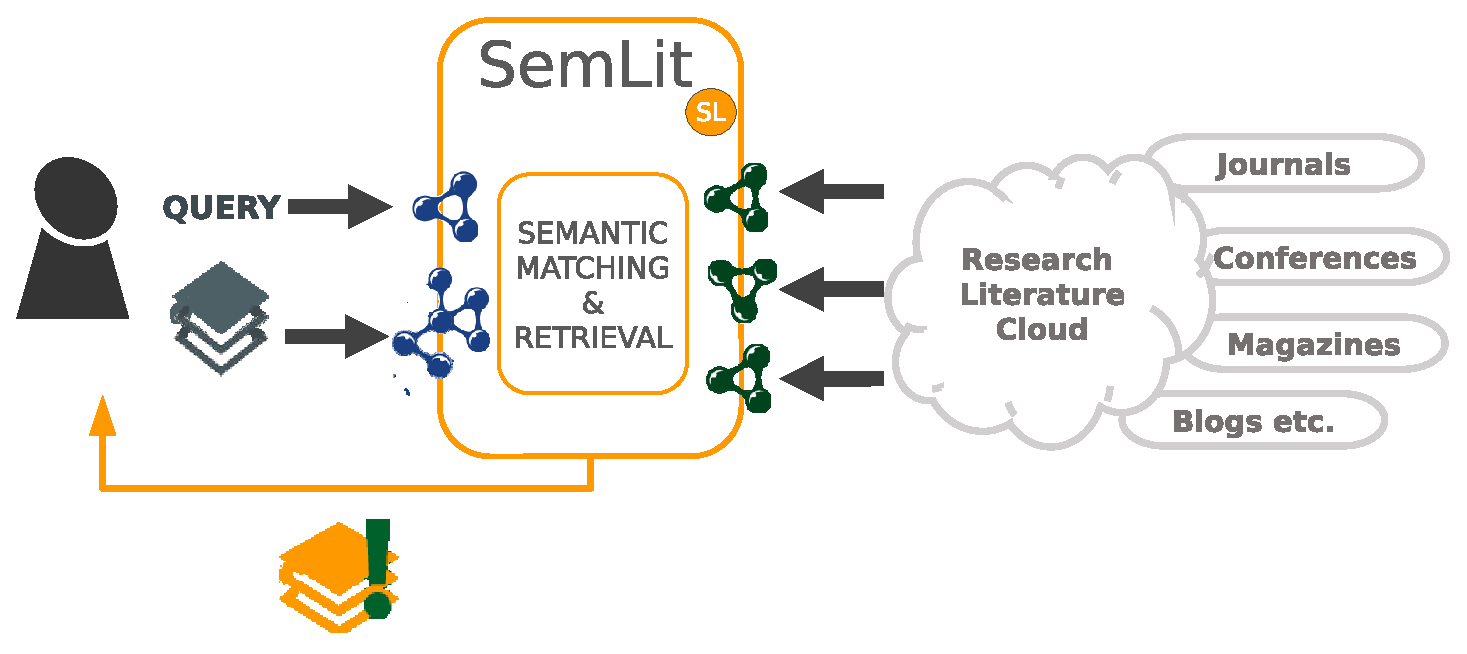
\includegraphics[width=0.9\textwidth]{idea}
\caption{Funktionsschema von SemLit}
\label{fig:financials2}
\end{figure}
